\chapter{Literature Review}
\label{cap:cap02}
 This section defines three main concepts in our research work: \acrshort{BNG} Protocol, another is the \acrshort{P4} language, the third MACSAD compiler and finally an ODP framework description.

\subsection{Broadband Access Networks}

 The first generation network based on centralizes BRAS routers was driven for the customer demand for High-speed Internet (HSI) the second generation Ethernet-based Broadband Network Gateway (BNG) routers was driven by subscriber demand for a linear TV service (content broadcast at specific times, e.g., Netflix) delivered in conjunction with voice and HSI services \cite{Alcatel}.\\
 The Customer Premise Equipment (CPE) represents the triple play communications devices: Telephone (Voice), PC (Internet), Set-top box (TV) however all these devices are connected to a Home Gateway (HG) that brings the interface with the network through any access technology like Digital Subscriber Line (DSL).\\
 One or more HG can be connected to a single DSLAM that sends the traffic to the BNG device and it route in a core IP network and the edge routers to provide connectivity to the Internet (See Figure \ref{fig:arch}).\\
 \begin{figure}[!h]
 	\centering
 	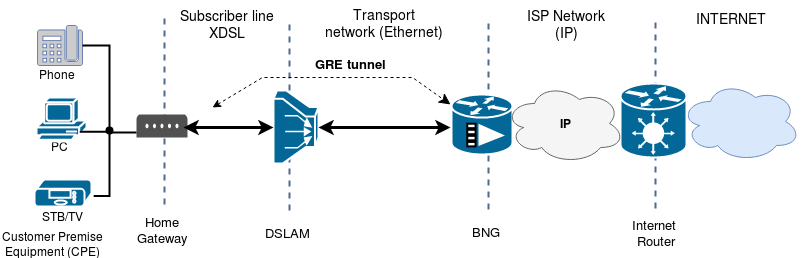
\includegraphics[width=0.8\linewidth]{figures/bng_architect.png}
 	\caption{Access Network Provider Model.}
 	\label{fig:arch}
\end{figure}
The network operator provides connectivity, authentication, applications and service network  policies to his users, therefore, these procedures involve the premise of session establishment using access communication protocols which are managed in the BNG, the most common protocols to establish session are:
\begin{itemize}
\item The PPP over Ethernet (PPPoE): Use the point-to-point (PPP) protocol.
\item The IP over Ethernet (IPoE): Use IP protocol that runs between CPE and BNG.
\item Generic Routing Encapsulation (GRE V2), encapsulation protocol brings virtual  Point-to-Point connections through IP network.
\end{itemize}
In our implementation, the packet sent or received by the HW are encapsulated with GRE headers, creating a point-to-point link with the BNG, but is just one of the options for packets encapsulation. \\
Since the BNG centralizes all the functions simplify the management functions like:
\begin{itemize}
\item Session management and header cap/decapsulation.
\item Interface to Authorization, Authentication and accounting services.
\item ARP proxy to manage the requests from the network interface on the BNG side.
\item Network Address translation to route the packets towards the operator’s core Network.
\item Interface to assignment queues and line rate to subscribers.
\end{itemize}
On the other hand, all these tasks make the structure of network rigid and become difficult to support the protocols and architectures in the current ISP.  In \cite{Rethinking} we found some similar approach to virtualize a Broadband Remote Access Server (BRAS) based on Click OS, a tiny Xen virtual machine designed specifically for network processing it can achieve line rate of 10Gbps and it composes of netmap and VALE as the packet I/O framework.
Our architecture approach goes with the same trend of network function virtualization using Macsad framework that compiles P4 code to bring more flexibility to the data plane and adding support for Hardware Abstraction Layer (HAL).\\
In the next session, we will describe our architecture design to be rapidly reconfigured using a “programming protocol-independent packet processors” (P4) and MACSAD to generate the datapath Logic codes.


% %%%%%%%%%%%%%%%%%%%%% subSection 2 P4 %%%%%%%%%%%%%%%%%%%%%%%%%%%%%%%%%%%
\subsection{Programming Protocol-Independent Packet Processors (P4)}
\begin{figure}[!h]
	\centering
	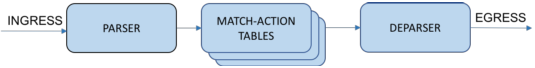
\includegraphics[width=0.7\linewidth]{figures/p4_dp.png}
	\caption{P4 Abstract Forwarding Model. Source: Adapted from \cite{P4}.}
	\label{fig:p4_dp}
\end{figure}
P4 is a high-level language for programming protocol-independent packet processors that define how the pipeline of a network forwarding device should process the packets using the abstract forwarding model (See figure \ref{fig:p4_dp}). P4 define the header structures and use the parser to extracts the header fields. The pipeline is defined through a series of match-action tables, which execute one or more actions like packet forwarding, drop and so on.  This tables can be changed and accessed at "runtime" through a controller software to add, remove and modify table entries and finally, de-parser writes the header fields back before sending the packets to the output port. The three main advantages of P4 are:

\begin{enumerate}
\item Reconfigurability in the field: Programmers should be able to change the way how the switch process the packets once that was deployed. 
\item Protocol independence: Capability to deploy any protocol in a switch.  
\item Target independence: To describe packet-processing functionality independent of the hardware where it has been deployed \cite{P4}.
\end{enumerate}

% %%%%%%%%%%%%%%%%%%%%% subSection 2 MACSAD %%%%%%%%%%%%%%%%%%%%%%%%%%%%%%
\subsection{Multi-Architecture Compiler System for Abstract Dataplanes (MACSAD)} 
\label{sec:Macsad}
This tool brings an environment to compile and deploy switch for L2/L3 applications automatically generating the datapath code for heterogeneous targets over 10Gbps network interfaces setup \cite{Patra}.\\
The MACSAD architecture is designed around the following three modules: (See the figure 2a) \\ \\
\begin{figure*}[!ht]
	\centering
	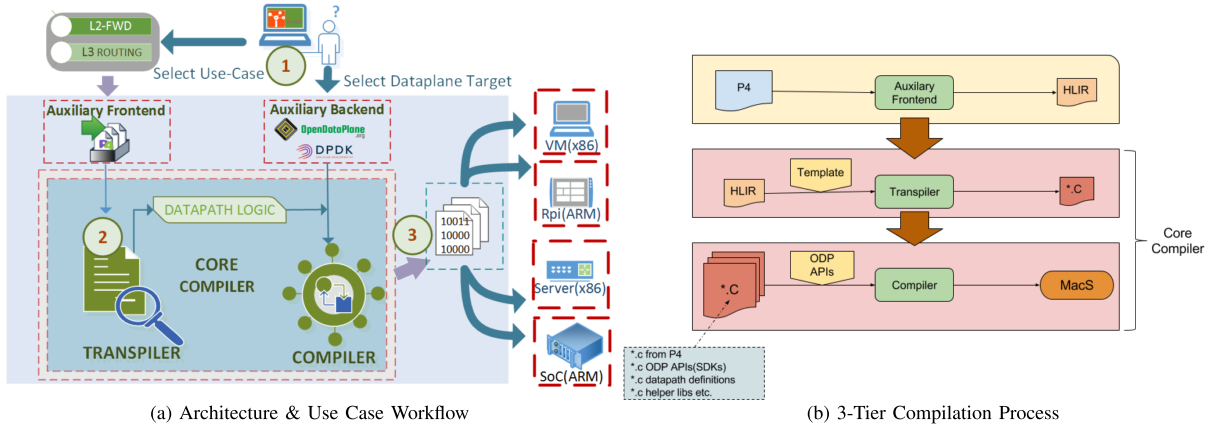
\includegraphics[width=0.85\linewidth]{figures/macsad_arch.png}
	\caption{Macsad architecture. Source:\cite{Patra}}
	\label{fig:mac_arch}
\end{figure*}

\textbf{- Auxiliary Frontend:} The P4 code is the MACSAD input that will be converted to an IR representation using the  p4-hlir framework that supports different Domain Specific Language (DSL) to generate a High-Level Intermediate Representation (HLIR) to be used in the Macsad core compiler.\\
\textbf{- Auxiliary Backend:} this module provides a common SDK for the Compiler incorporating the ODP APIs 
%  \cite{odp} 
 auto-generating support for different platforms with ODP supporting various control protocols like Switch Abstraction Interface (SAI), OpenFlow (OF), and other useful events for buffer like queueing, scheduling, etc.\\
\textbf{- Core Compiler:} Composed of a Transpiler and a Compiler submodule (see the figure \ref{fig:mac_arch}b), transforms the IR generated by the frontend into the target imaged in association with the auxiliary backend.\\
The transpiler takes the HLIR input and auto-generates the Datapath Logic codes. Some critical decision is taken in this sub-module like to optimize the ’Dead Code Elimination’ by identifying reachability in a graph, decides the type of look-up mechanism to be used, and size and type of tables to be created by. 
The Macsad compiler creates a set of libraries in 'C' codes for the desired target (x86, x86+DPDK, ARM-SoC).\\
The BNG P4 code will be added to the system as an input to create the BNG router. Also, Macsad tool brings the generation of high-level ODP APIs to deliver platform abstraction with high performance and hardware-acceleration options.



\subsection{Open Data Plane (ODP)}
Open Data Plane project provides an application programming environment for data plane applications with high performance and portable across a lot of HW platform.
The aim of ODP is separate application design from the functional implementation of that design, this because historically it requires that data plane application must be redesigned on changes in network speed and capacity because the applications need to be very integrated with specialized hardware to achieve acceptable performance levels.
ODP relies on the Linux kernel itself; it defines some ODP API set to rapid porting ODP application to any platform (See Figure \ref{fig:sys_arch}), it can define functions and limits like a number of queues or used cores processor.\\
% %%% -----------
\begin{figure*}[!ht]
	\centering
	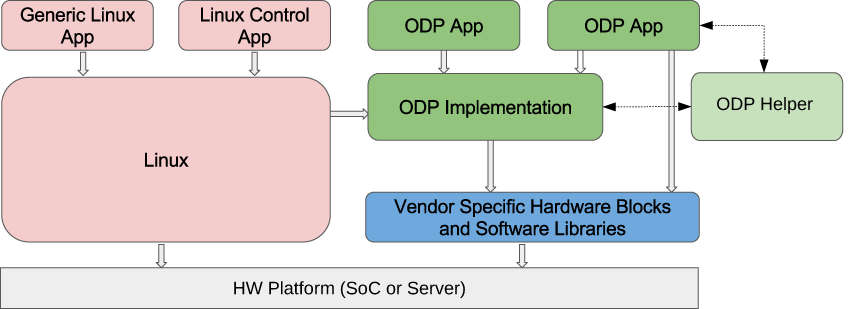
\includegraphics[width=0.6\linewidth]
     {figures/odp-overview.png}
% 	\caption{ODP system architecture. Source:\cite{opd_spec}}
 	\caption{ODP system architecture. Source:....}
	\label{fig:sys_arch}
\end{figure*}
ODP applications can run in parallel with full Linux user processes that implement control and management functions since that these typically do not have critical performance and latency requirements. In that sent, this tool calls the Software Development Kit (SDK) and optimize the features and functionalities for the particular hardware platform (SoC or Server).
The ODP APIs is written in the C programing language and are optimized to control related SoC resources such as:
\begin{itemize}
\item CPUs (or hardware threads) 
\item Main memory
\item Huge page mappings (how many, what sizes) 
\item Physical and virtual ports/interfaces 
\item Packet classification rules 
\item Scheduler (core groups, algorithms, ordering) 
\item Hardware queues 
\item Output traffic management 
\item hardware Quality of Service (QoS) support. 

\end{itemize}


